\documentclass[onecolumn]{article}
\usepackage{mathpazo}
\usepackage{microtype}
\usepackage{graphicx}
\usepackage{amssymb}
\usepackage{amsmath}                     %%
\usepackage{amsfonts}                    %%  for AMS mathematics
\usepackage{amsthm}
\usepackage{algorithmic}
\usepackage{algorithm}
\usepackage{url}
\usepackage{natbib} 

\setlength\textwidth{7in} 
\setlength\textheight{9.5in} 
\setlength\oddsidemargin{-0.25in} 
\setlength\topmargin{-0.25in} 
\setlength\headheight{0in} 
\setlength\headsep{0in} 
\setlength\columnsep{18pt}
\sloppy 

%%%%% +++++++++++++++ wsun, 5/15/10 %%%%%%%%%%%%%%%%%%%%%%%%
%%%%% add the following to make environment definition, theorem, etc. %%%%%%%%%%%%%
\newtheorem{definition}{Definition}
\newtheorem{theorem}{Theorem}
\newtheorem{proposition}{Proposition}
\newtheorem{example}{Example}

 
\begin{document}

\title{
\vspace{-0.5in}\rule{\textwidth}{2pt}
\begin{tabular}{ll}\begin{minipage}{4.75in}\vspace{6px}
\noindent\LARGE Center of Excellence in C4I\\
\vspace{-12px}\\
\noindent\large George Mason University\qquad Technical Reports
\end{minipage}&\begin{minipage}{2in}\vspace{6px}\small
4400 University Drive MS\#4A5\\
Fairfax, VA 22030-4444 USA\\
http:/$\!$/c4i.gmu.edu/\quad 703-993-5538
\end{minipage}\end{tabular}
\rule{\textwidth}{2pt}\vspace{0.25in}
\LARGE \bf
Dynamic Asset Cluster Model, a Trade-Based Asset Model using Junction Tree Structure, with interval questions, for Combinatorial Prediction Markets
}

\date{Technical Report (March, 2014)
%\#\#\#
}

\author{
{\bf Wei Sun}\\
wsun@c4i.gmu.edu
%\and 
%{\bf SECOND AUTHOR NAME (AND SO ON)}\\
%SECOND AUTHOR EMAIL ADDRESS
}

\maketitle

\begin{abstract}
\textbf{CONFIDENTIAL}: This is the internal documentation of implementing DAC (Dynamic Asset Cluster) model with interval questions, for combinatorial prediction markets. The implementation is coded in Matlab.
\end{abstract}

\section{Prerequisites}
\label{sec:pre}

In our context, basically we partition the continuous values state space of the variable into dynamically changing set of intervals, so we call an interval question value-partitioning node (VP-node). It is not real continuous variables in our current application yet. We assume that there are a set of atomic units as the lowest level elements (sometimes called leaf in hierarchy) for any VP-node. When we partition values for a VP-node, we mean to group corresponding atomic units into an interval or range. \\[1pt]

In general, a trade involving a VP-node has to define its reference range ($rr$) and target range ($tr$). By default, $rr$ is the entire value set of the VP-node. \\[1pt]

We maintain a data structure for representing a VP-node, in which we have attributes called `min', `max' for representing its whole value set, `cutpoints' to save all cutting points in between `min' and `max' but not including them. `cutpoints' needs to be updated after any interval trades. Consequently, number of states for the VP-node, a.k.a. node size, can be derived by counting cutting points + 1. \\[1pt]

We maintain a \textit{DAC} asset structure for any user who has at least one trade. \textit{DAC} has following attributes: (1)$base$--base asset, which is initial asset + manna + realized gain/loss; (2)$Obj\_list$--Object list; (3)$Q\_list$--question list; (4)$ns$--node sizes; (5)$abc$--asset blocks collection.  \\[1pt]

Whenever there is a trade involving a VP-node, we need to update \textit{DAC} model by updating all asset blocks containing the corresponding VP-node. Arguments needed for the function are: 
\begin{enumerate}
	\item current \textit{DAC}; 
	\item involving VP-node; 
	\item asset change $delta$, which is always a vector of two values; 
	\item $tr$, target range; 
	\item $rr$, reference range (optional); 
	\item regular assumption questions (optional); 
	\item given states of regular assumption questions (optional); 
	\item node sizes of regular assumption questions (optional); 
	\item conditioning VP-node (optional); 
	\item given range of conditioning VP-node (optional).
\end{enumerate}


\section{Test Cases \& Implementations} \label{sec:testcase}

\subsection{Case 1: a trade on the target range only for a VP-node $p(tr)$}
Suppose a VP-node called \textit{RainVP} has its atomic units represented by integers from 1 to 19 as its entire value set. \textit{Rain} has uniform prior $p0$. The trade is, without specifying any reference range (by default, $rr$ is the entire value set), to decrease the current probability over the range of $[3,10]$ from about $0.421053$ by 15\%, namely, to lower down to about  $0.357895$. We then proportionally assign updated probabilities to individual atomic units.  Particularly, updated probability distribution for \textit{RainVP} after the trade is $p1=[0.0584, 0.0584, 0.0447, 0.0447, 0.0447, 0.0447, 0.0447, 0.0447, 0.0447, \\0.0447, 0.0584, 0.0584, 0.0584, 0.0584, 0.0584, 0.0584, 0.0584, 0.0584, 0.0584]$. Accordingly, \textit{RainVP} has cutpoints \{$3,10$\} partitioning its state set into $3$ bins, namely, $[1,3]$, $[3,10]$, and $[10, 19]$. Correspondingly, asset changes in those bins are shown in Figure \ref{fig:assetchange1}.

\begin{figure}[tbh]
    \centering    
    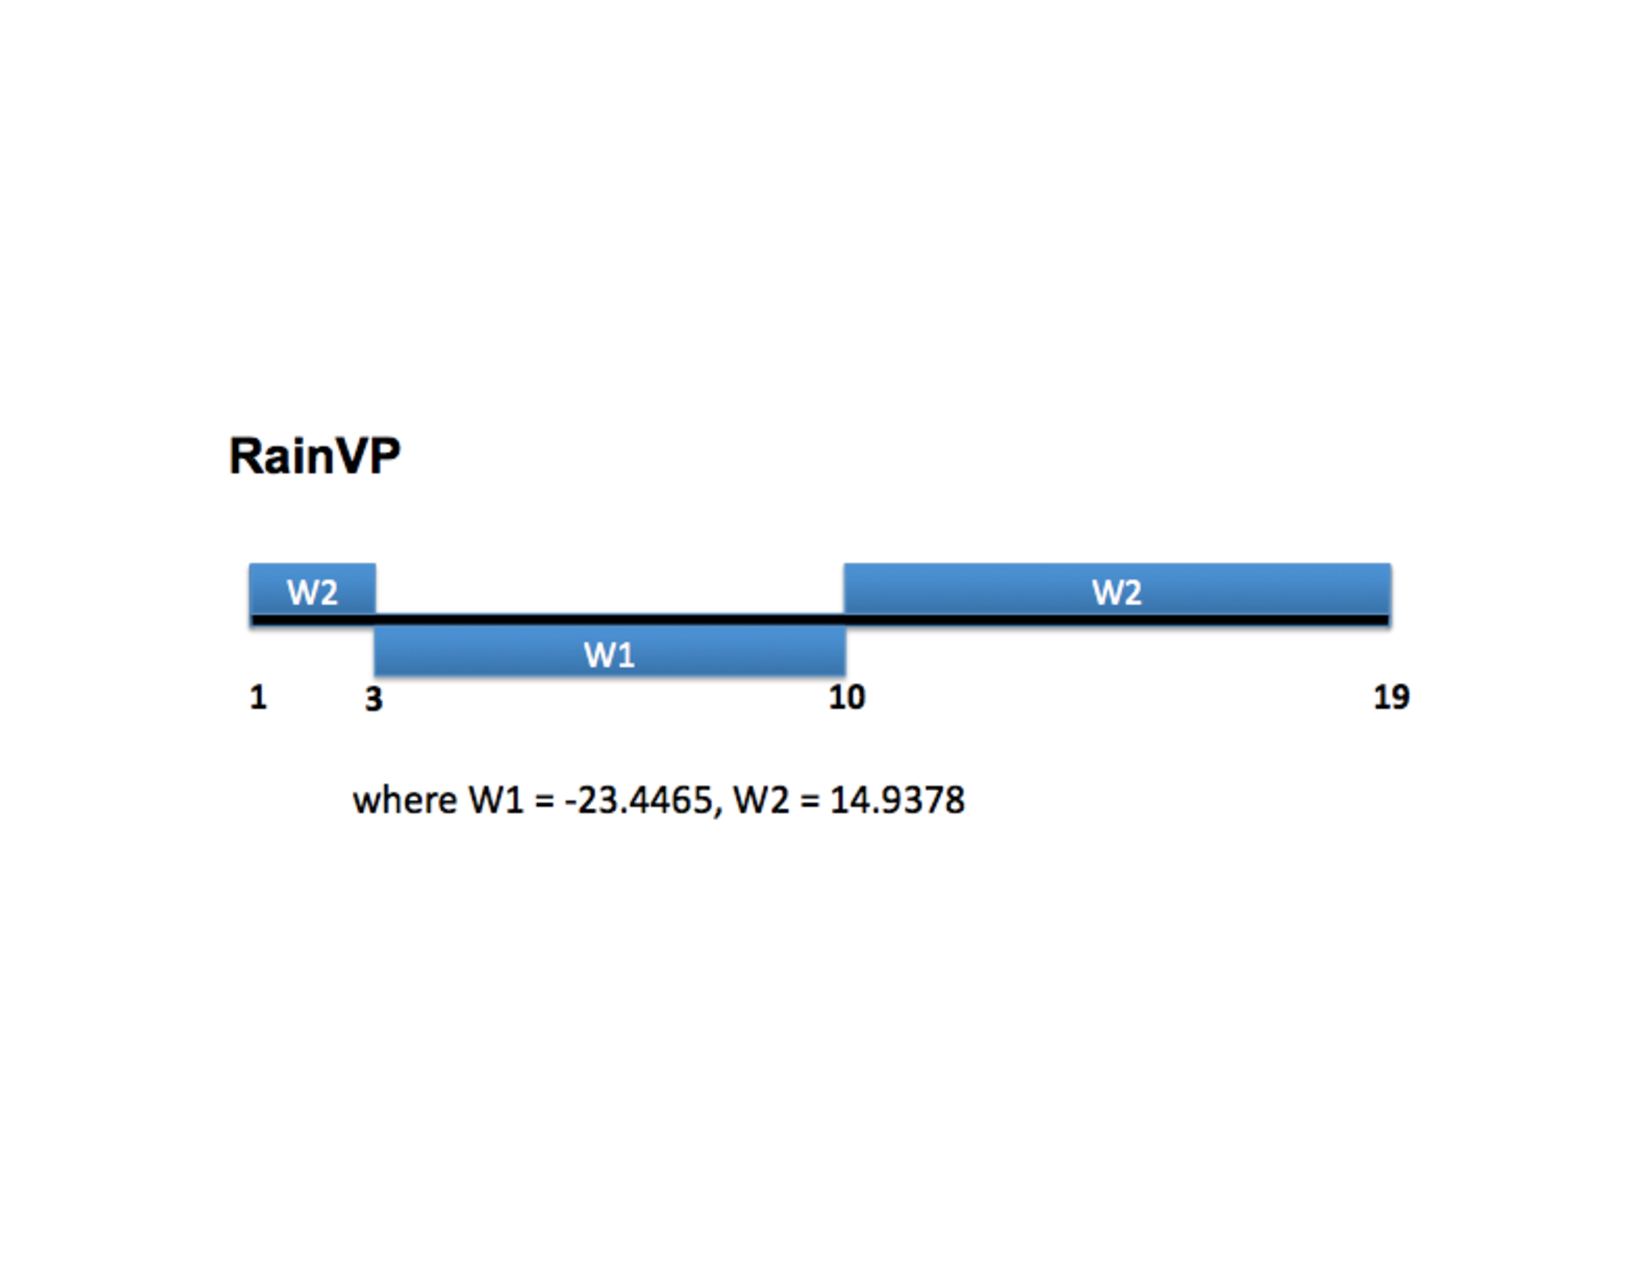
\includegraphics[scale=0.65]{DAC_VP_figure/assetchange1_rainVP.pdf}     
    \caption{Asset changes distribution on \textit{RainVP}} 
    \label{fig:assetchange1} 
\end{figure}


\subsection{Case 2: a trade on the target range given a reference range for a VP-node $p(tr|rr)$}
We conduct the second trade on \textit{RainVP} again. This time we specify a reference range as $[5,13]$, then trade on the target range of $[8,9]$. Specifically, the trade is to raise up by $25\%$ on the base of the current probability of the interval of $[8,9]$ given $[5,13]$. After the trade, the updated probability distribution for \textit{RainVP} becomes $p2=[0.0584, 0.0584, 0.0447, 0.0447, 0.0419, 0.0419, 0.0419, 0.0559, 0.0559, 0.0419, 0.0547, 0.0547, 0.0547, 0.0584, 0.0584, 0.0584, \\0.0584, 0.0584, 0.0584]$. And \textit{RainVP} has new partition sets as $[1,3]$, $[3,5]$, $[5,8]$, $[8,9]$, $[9,10]$, $[10, 13]$, and $[13, 19]$. The new trade resulted in new asset changes over new generated bins of $[5,8]$, $[8,9]$, $[9,13]$, illustrated in Figure \ref{fig:trade2} as $W3$, $W4$:

\begin{figure}[tbh]
    \centering    
    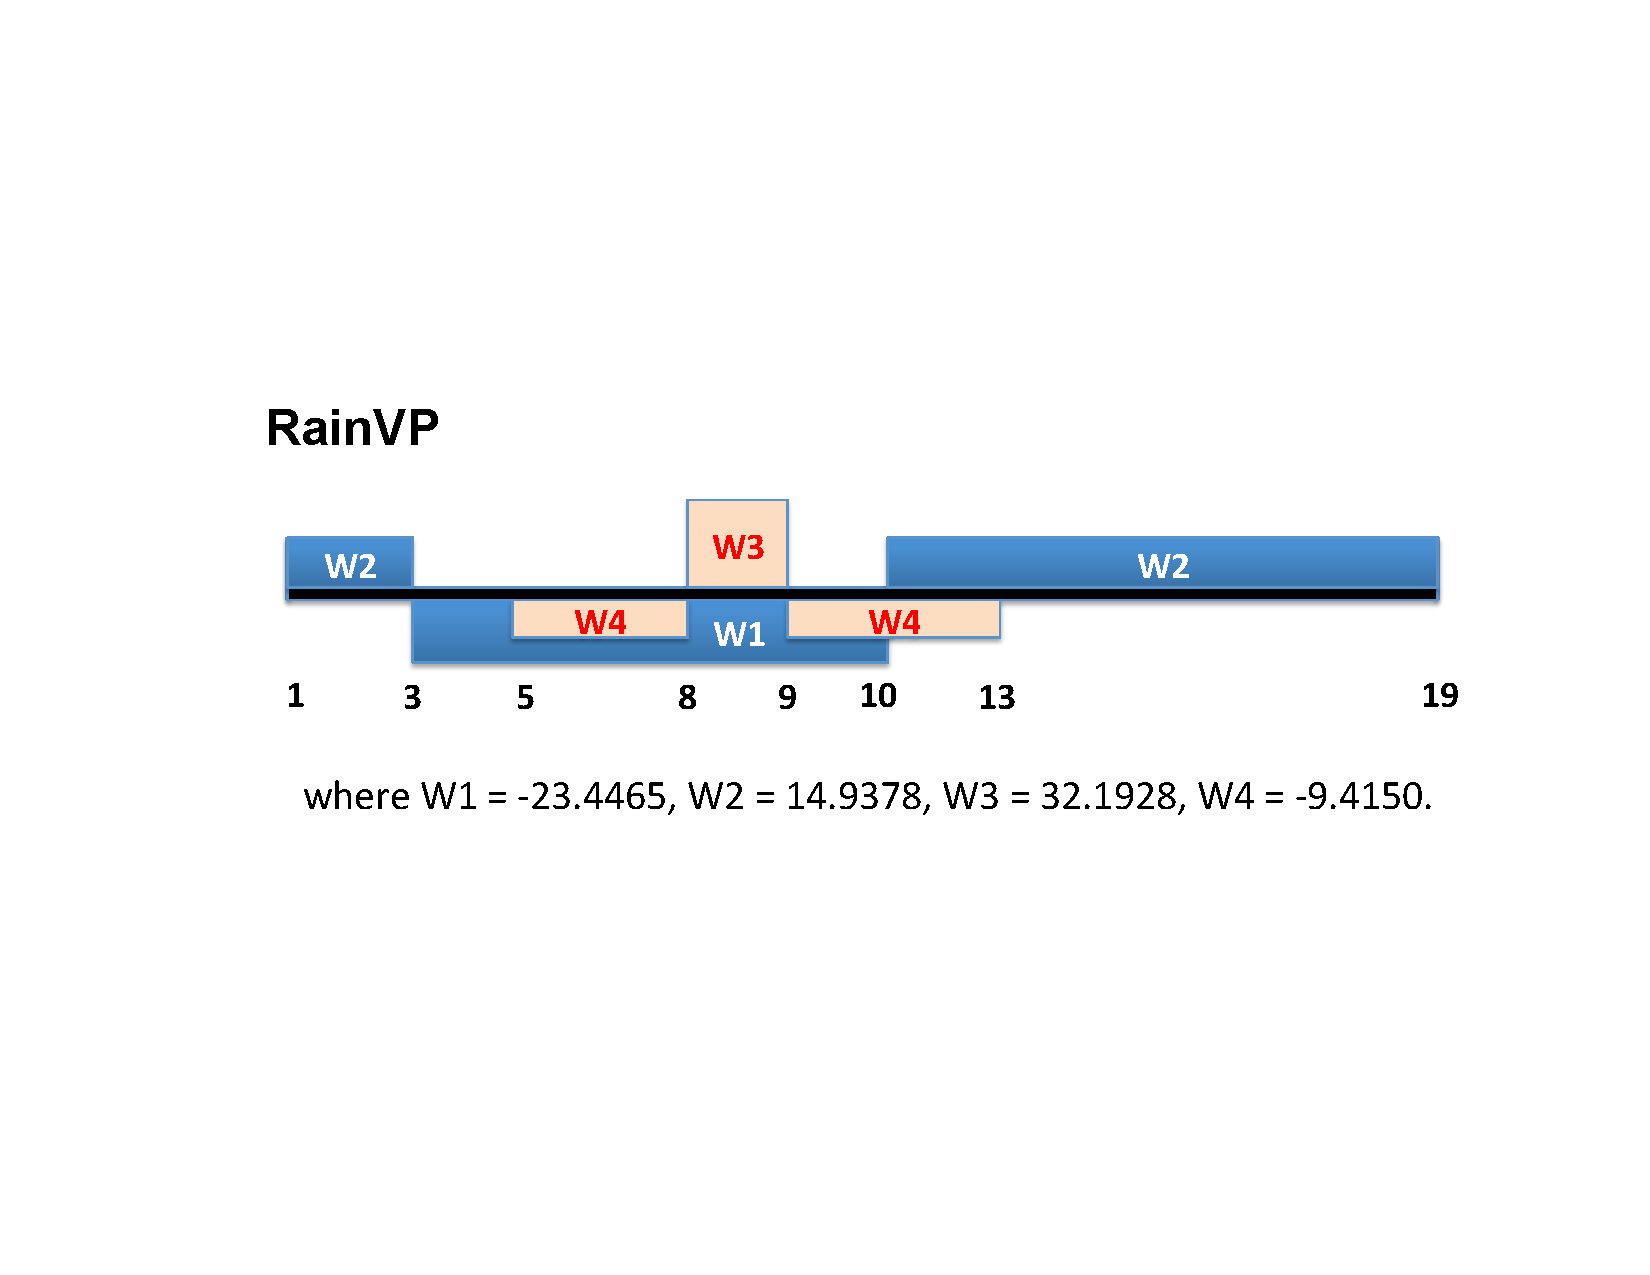
\includegraphics[scale=0.65]{DAC_VP_figure/trade2_rainVP.pdf}     
    \caption{Asset changes over newly generated bins of \textit{RainVP}} 
    \label{fig:trade2} 
\end{figure}

Please note the old asset gain/loss generated by the first trade have not been combined yet. After aggregation, we have new set of bins and corresponding asset changes shown in Figure \ref{fig:assetchange2}:

\begin{figure}[tbh]
    \centering    
    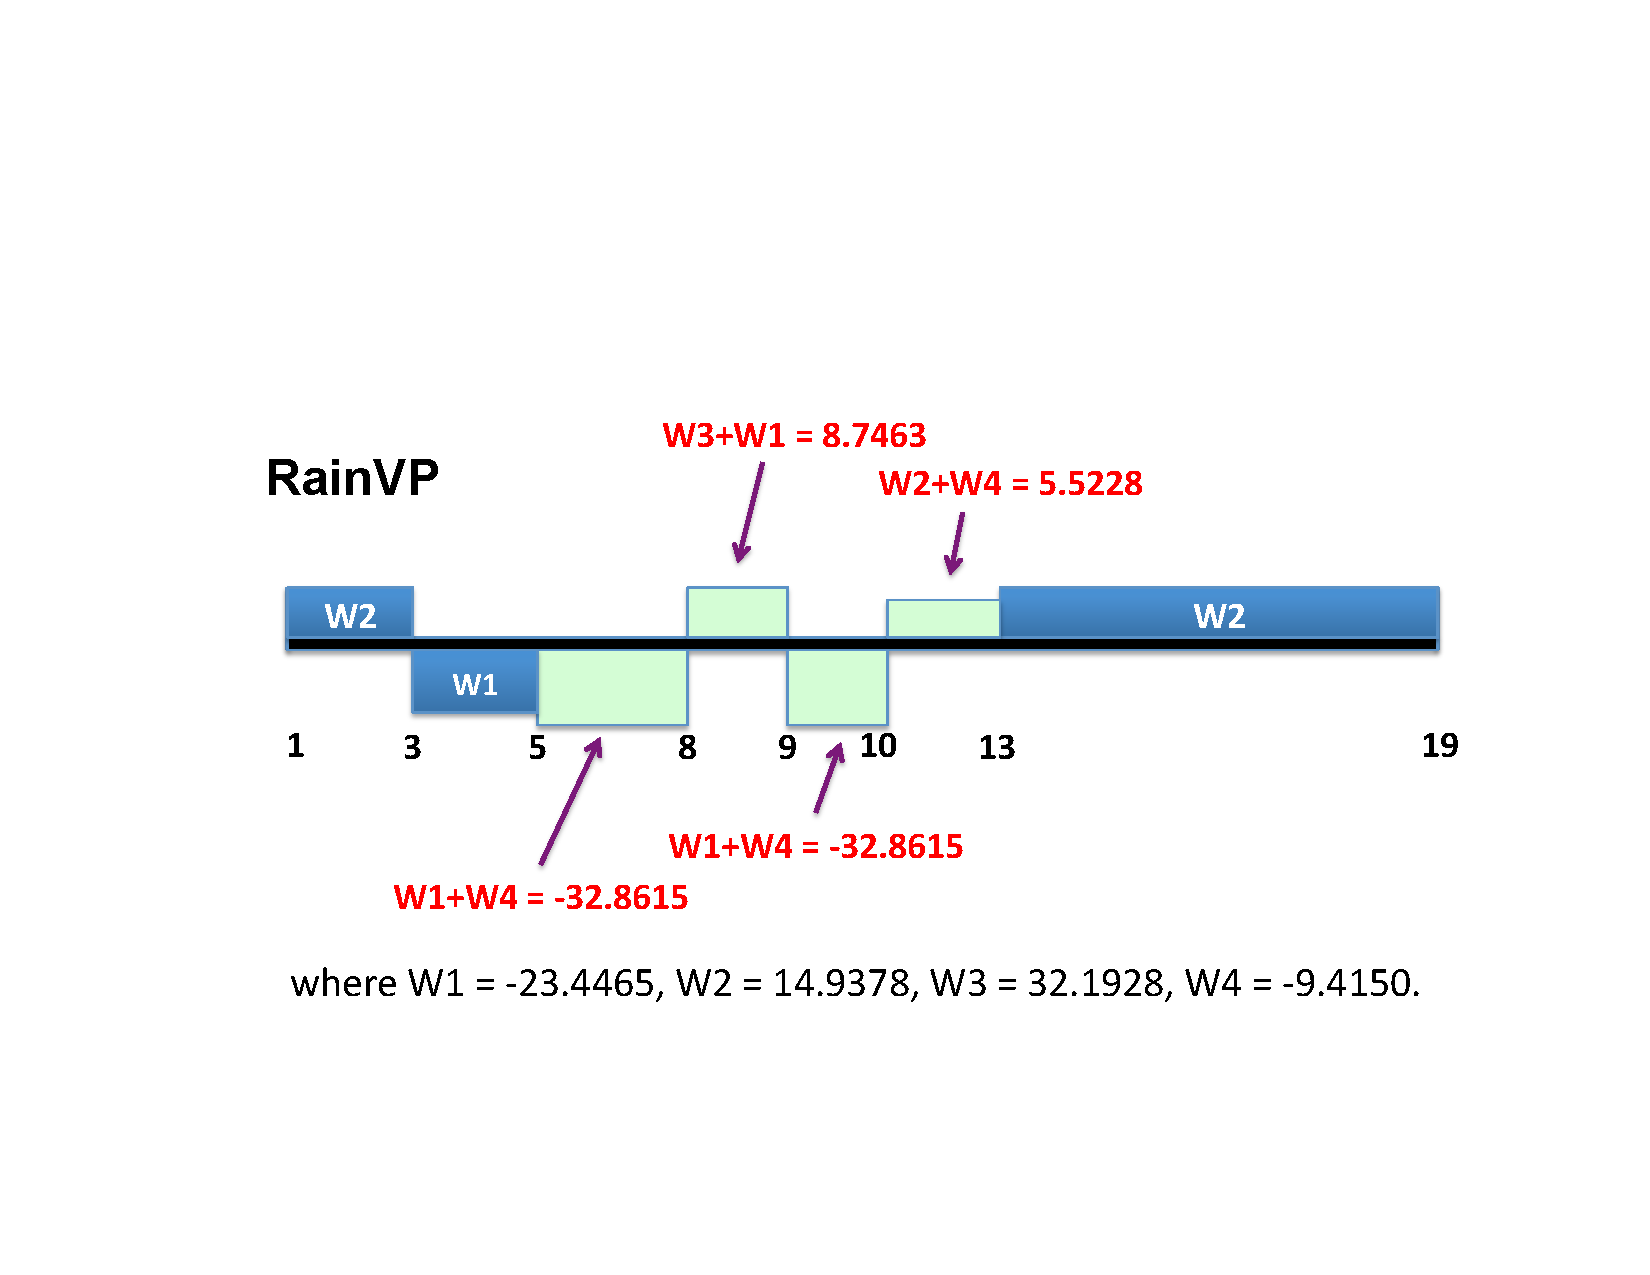
\includegraphics[scale=0.65]{DAC_VP_figure/assetchange2_rainVP.pdf}     
    \caption{New asset distribution of \textit{RainVP}} 
    \label{fig:assetchange2} 
\end{figure}

\subsection{Case 3: trade on the target range of a VP-node given its reference range and another regular assumption question $p(tr|rr, A)$}
Now let consider the case when trading on the target range of a VP-node given its reference range and another regular assumption question $p(tr|rr, A)$. 


\subsection{Case 4: $p(tr|rr, VP\_A)$}
I made a Netica BN model consisting of one VP-node called $sand\_VP$(integers from 1 to 10 as its atomic units), and a regular two-state question $A$ as one of parent of $sand\_VP$, and a VP assumption question, called $VP\_A$ (integers from 1 to 4 as its atomic units), as another parent of $sand\_VP$. \\[2pt]


\newpage
\textbf{The rest of paper from this page are just the backup for LaTeX formulas. Please ignore contents from this page.}
\begin{eqnarray*} \label{eqn_pfactor}
 p'(D,E,F) &=& \frac{p'(D,E) \times p'(D,F)}{p'(D)} \\
              &=& p'(D,E) \times p'(F|D) \\
              &=& p'(D,E) \times p(F|D) \\
              &=& p'(D,E) \times \frac{p(D,F)}{p(D)} \\
              &=& \frac{p'(D,E) \times p(D,F)}{p(D)} 
\end{eqnarray*} 



\begin{table}
\label{tab:mpprotocol}
\caption{Customized min-propagation protocol for asset junction tree}
\small
\hrulefill
\begin{enumerate}
  \item Let ${\phi(\mathbf{S}_{ij})}' =  \min_{\mathbf{C}_i \backslash
  \mathbf{S}_{ij}} \phi(\mathbf{C}_i)$, ---  minimalizng the
  potential $\phi(\mathbf{C}_i)$ onto the domain of  separator
  $\phi(\mathbf{S}_{ij})$, i.e., finding the minimum values over the dimensions of minimalized variables and then projecting them to the domain of separator.
  \item Let $\mathcal{L}(\mathbf{S}_{ij}) = {{\phi(\mathbf{S}_{ij})}'} -  {\phi(\mathbf{S}_{ij})}$,  --- subtracting the old asset in the separator $\mathbf{S}_{ij}$ from its new values. The resulting value is called the separator gain, because it filters out the overlapping information between the sending clique and the separator. 
  %The ratio $\mathcal{L}(\mathbf{S}_{ij})$ is served as 
  %information ratio, also called "likelihood ratio", to update
  %information by filtering out the redundant part.
  %\item Let $\phi(\mathbf{S}_{ij}) = {\phi(\mathbf{S}_{ij})}'$,  ---
  %storing the new potential of the separator for next round message passing.
  \item Let $\phi(\mathbf{C}_j) = \phi(\mathbf{C}_j) + \mathcal{L}
  (\mathbf{S}_{ij})$, --- summing up with the separator gain to update the asset of $\phi(\mathbf{C}_j)$ .
\end{enumerate}
\hrulefill
\end{table}

\begin{equation}
  \label{eqn:editlimits}
  \left[ {p(T=t|\mathbf{A=a})}exp(\frac{-m_t}{b}), 1- (1-p(T=t|\mathbf{A=a}))exp(\frac{-m_{\neg t}}{b}) \right] . 
\end{equation}

\textbf{Asset update} - Once we have defined the joint asset over disconnected networks as shown above, we can do the following after making edit on probabilities:
\begin{eqnarray}
    S'({\cal{A,B,C}}) &=& S({\cal{A,B,C}}) + b * log(\frac{p'({\cal{A}})*p'({\cal{B}})*p'({\cal{C)}}}{p({\cal{A}})*p({\cal{B}})*p({\cal{C)}}}) \nonumber \\
                   &=& S({\cal{A}})+ S({\cal{B}}) + S({\cal{C}}) - S({\cal{AB}}_0) - S({\cal{BC}}_0) + b*log(\frac{p'({\cal{A}})}{p({\cal{A}})} + b*log(\frac{p'({\cal{B}})}{p({\cal{B}})} + b*log(\frac{p'({\cal{C}})}{p({\cal{C}})} \nonumber \\
                   &=& S'({\cal{A}})+ S'({\cal{B}}) + S'({\cal{C}}) - S({\cal{AB}}_0) - S({\cal{BC}}_0)
\end{eqnarray}


\textbf{Soft Evidential Update}: Jeffurey rule.
Suppose we have a joint distribution over four variables $T$,$W$,$X$, and $Y$. Suppose we have current joint probability over these four variables as $P(T,W,X,Y)$. No matter what edit the user likes to do, all of other conditional probabilities should remain same. Essentially, the edit is just a partial change over the original probability space. Let us have an example to show how to do soft evidential update over the joint space. Assuming we have an edit on $T$ given $X$, $Q(T|X)$, then the new joint probability will be 

\begin{eqnarray*}
	P'(T,W,X,Y) &=& P'(W|T,X,Y)*P'(Y|T,X)*P'(T|X)*P'(X) \\
                    &=& P(W|T,X,Y)*P(Y|T,X)*Q(T|X)*P(X)  \\
                    &=& P(T,W,X,Y) * \frac{Q(T|X)}{P(T|X)}  
\end{eqnarray*}
The key is that we can shuffle the order of variables in the chain rule to always make the one being edited separated out as one term, and all of other terms remain same. And of course, we can always calculate the curren probability of the coming edit from the joint, which is $P(T|X)$ in the example above.
\begin{equation}
    v(x) = \sum_{i=1}^{N} (K(x_i)) / N
\end{equation}



\bibliographystyle{apa}
\bibliography{markovEngine_uai2012}

\end{document}
